\documentclass{article}
\usepackage{graphicx}
\usepackage{amsmath}

\title{The Boat kata}
\author{Jarosław Karczmarczyk}
\date{}

\begin{document}
\pagestyle{empty}
\begin{center}
  \section*{The Boat kata}
\end{center}

\noindent Let’s imagine that you’re designing a part of a boat navigation system. The boat is moving from one point to another along a line. It is possible to change the course only at each point. The goal is to determine whether the boat is facing left or right. The boat is facing right if and only if the sum of angles of turns is greater than zero. Each turn is always represented by the smallest possible angle. Assume that whenever the boat is turning right then the sign of the turn's angle is positive and negative otherwise.
\begin{figure}[htpb]
\begin{center}
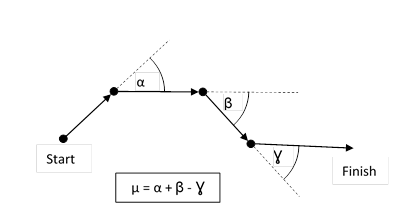
\includegraphics{boat_path.png}
\caption{Boat turns and sum of all the angles}
\label{fig:boat_path}
\end{center}
\end{figure}

\noindent In Fig.~\ref{fig:boat_path} sum of angles is denoted by $\mu$ and when it is greater than zero then boat is facing right. 

\subsection*{Input}
The input consists of two lines. First line contains one integer ($0 \leq n \leq 1000000$) which is always even. This is the number of numbers in second line. 
The second line contains a sequence of pairs of numbers describing consecutive points of the boat's path. In each pair, the first number ($0 \leq x \leq 1 000 000$) is the X coordinate and the second number ($0 \leq y \leq 1 000 000$) is the Y coordinate.

\subsection*{Output}
Output contains always only one word: ``True'' or ``False''.
If it is possible to determine whether the boat is facing right and if it is facing right, then in the output should be ``True''. Otherwise, the output should be ``False''.
\end{document}
